\documentclass[border=4pt]{standalone}
\usepackage{tikz}
\usetikzlibrary{calc}
\usepackage{pgfplots}
\pgfplotsset{compat=1.18}
\usepgfplotslibrary{fillbetween}
\usepackage{amsmath}
\usepackage{libertine}
\usepackage{xcolor}
\definecolor{charcoal}{HTML}{2D3748}
\definecolor{forest}{HTML}{2B6CB0}
\definecolor{warmgray}{HTML}{718096}
\definecolor{harvardcrimson}{HTML}{A51C30}
\definecolor{seagreen}{HTML}{2F855A}

% What limits tag tracking, III: edge-on. The height in pixels of a row of cells at
% the tag's far edge as the tag turns from face-on towards edge-on, for three tag
% sizes in the image (three distances of a 0.10 m tag with f = 800 px). Every row
% is foreshortened by cos(theta); the far rows are also farther away by (d/2) sin(theta):
%   h_row = (s/8) cos(theta) * z / (z + (d/2) sin(theta)),   s = f d / z.
% Pure geometry, no data file. The grey band marks cells narrower than about
% 2 px, roughly twice a typical lens blur, which a detector cannot read.
%   pdflatex limit-oblique.tex && pdftocairo -svg limit-oblique.pdf ../figures/limit-oblique.svg
\def\f{800} \def\dd{0.1}

\begin{document}
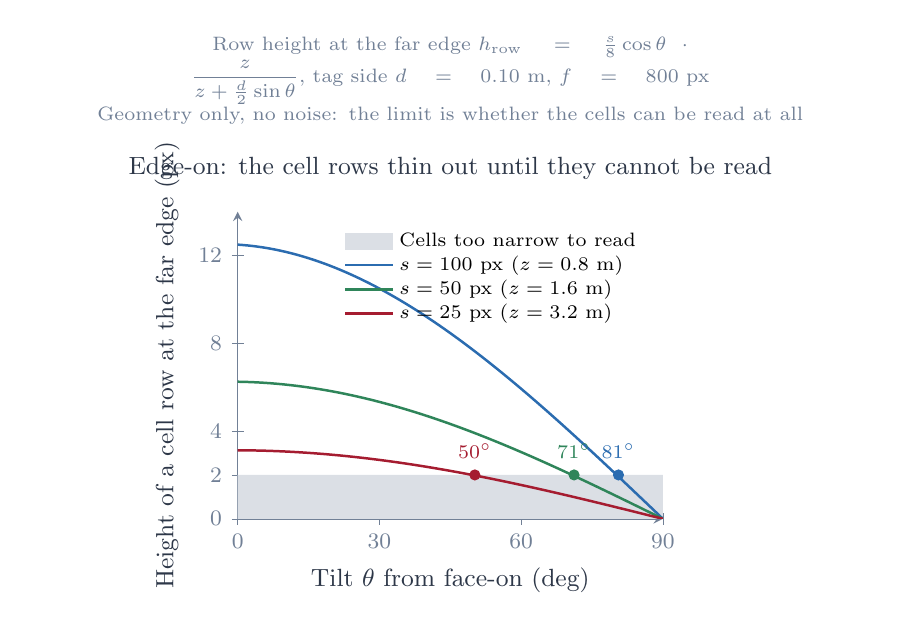
\begin{tikzpicture}[font=\small]
  \begin{axis}[
      scale only axis, width=5.4cm, height=3.9cm, name=panel,
      axis line style={warmgray, line width=0.5pt},
      tick style={warmgray}, ticklabel style={font=\footnotesize, color=warmgray},
      label style={font=\small, color=charcoal},
      title style={font=\small, color=charcoal, yshift=2pt},
      legend style={draw=none, fill=none, font=\scriptsize, at={(0.97,0.97)}, anchor=north east, cells={anchor=west}, row sep=-2pt},
      axis x line=bottom, axis y line=left,
      xmin=0, xmax=90, xtick={0,30,60,90},
      ymin=0, ymax=14, ytick={0,2,4,8,12},
      xlabel={Tilt $\theta$ from face-on (deg)},
      ylabel={Height of a cell row at the far edge (px)},
      title={Edge-on: the cell rows thin out until they cannot be read},
      domain=0:90, samples=120]
    % the unreadable band: cells narrower than about 2 px
    \addplot[name path=floor, draw=none, forget plot] {2};
    \addplot[name path=zero, draw=none, forget plot] {0};
    \addplot[warmgray!25] fill between[of=floor and zero];
    \addlegendentry{Cells too narrow to read}
    % one curve per tag size: s = 100, 50, 25 px, i.e. z = 0.8, 1.6, 3.2 m
    \addplot[forest, line width=0.9pt]         {(100/8)*cos(x)*0.8/(0.8 + 0.05*sin(x))};
    \addlegendentry{$s = 100$ px ($z = 0.8$ m)}
    \addplot[seagreen, line width=0.9pt]       {(50/8)*cos(x)*1.6/(1.6 + 0.05*sin(x))};
    \addlegendentry{$s = 50$ px ($z = 1.6$ m)}
    \addplot[harvardcrimson, line width=0.9pt] {(25/8)*cos(x)*3.2/(3.2 + 0.05*sin(x))};
    \addlegendentry{$s = 25$ px ($z = 3.2$ m)}
    % where each curve enters the band
    \addplot[forest, only marks, mark=*, mark size=1.8pt, forget plot] coordinates {(80.6, 2)};
    \node[forest, anchor=south, font=\scriptsize] at (axis cs:80.6, 2.3) {$81^\circ$};
    \addplot[seagreen, only marks, mark=*, mark size=1.8pt, forget plot] coordinates {(71.2, 2)};
    \node[seagreen, anchor=south, font=\scriptsize] at (axis cs:71.2, 2.3) {$71^\circ$};
    \addplot[harvardcrimson, only marks, mark=*, mark size=1.8pt, forget plot] coordinates {(50.2, 2)};
    \node[harvardcrimson, anchor=south, font=\scriptsize] at (axis cs:50.2, 2.3) {$50^\circ$};
  \end{axis}
  % the set-up, above the panel, so the figure can stand on its own
  \node[anchor=south, font=\scriptsize, text=warmgray, align=center, text width=10.5cm] at ($(panel.north west)!0.5!(panel.north east)$) [yshift=28pt]
    {Row height at the far edge $h_{\mathrm{row}} = \tfrac{s}{8}\cos\theta \cdot \dfrac{z}{z + \tfrac{d}{2}\sin\theta}$, tag side $d = 0.10$ m, $f = 800$ px\\
     Geometry only, no noise: the limit is whether the cells can be read at all};
\end{tikzpicture}
\end{document}
